\documentclass[9]{beamer}
\usepackage{beamerthemesplit}
\mode<presentation>
{
  \usetheme{Warsaw}
  % or ...

  \setbeamercovered{transparent}
  % or whatever (possibly just delete it)
}
%\setbeameroption{show notes}

\usepackage[english]{babel}
\usepackage[latin1]{inputenc}

\usepackage{times}
\usepackage[T1]{fontenc}

% \documentclass{elsart}
% \documentclass[doublespacing]{elsart}
\usepackage{graphicx}
\usepackage[nogin]{Sweave}
\usepackage[numbers]{natbib} \bibliographystyle{plainnat}
\usepackage{amsmath}
\usepackage{amssymb}
\usepackage{yfonts}
\usepackage{amsfonts}
%\usepackage{subfig}
\usepackage{tabls}
\usepackage{url}
\usepackage{pslatex}
\usepackage{makeidx}
\usepackage{dchem}
\usepackage{color}

\newcommand{\deriv}[2]{\ensuremath{\frac{\mathrm{d} #1}{\mathrm{d} #2}}}

\title{Statistical Modeling of Biochemical Pathways}
\author{Robert B. Burrows\inst{1} \and Gregory R. Warnes\inst{2,3} }
\institute{ 
  \inst{1}%
  New England Biometrics\\
  North Scituate, RI
  \and
  \inst{2}%
  Statistical Applications \\
  Pfizer, Inc.
  \and
  \inst{3}%
  Department of Computer Science \\
  Yale University
}

\begin{document}

\note{
$ $Id$ $
}

%\begin{abstract}
%The usefulness of Markov chain Monte Carlo methods for the modeling
%of biochemical reactions is examined. With simulated data, it is
%shown that mechanistic models can be fit to sequences of enzymatic
%reactions. These methods have the advantages of being relatively easy
%to use and producing probability distributions for the model
%parameters rather than point estimates.

%Three Markov chain Monte Carlo algorithms are used to fit models to
%data from a
%sequence of 4 enzymatic reactions. The algorithms 
%are evaluated with respect to
%the goodness-of-fit of the fitted models and the time to completion.
%It is shown that the algorithms produce essentially the same
%parameter distributions but the time to completion varies. 
%\end{abstract}

\frame{
  \maketitle
}

\section[Outline]{}
\frame{
  \frametitle{Outline}
  \tableofcontents
}

\section{Overview}
\frame{
  \frametitle{Overview}
  \begin{block}{Goal:}
    Estimate key rate parameters of biological pathways, e.g

    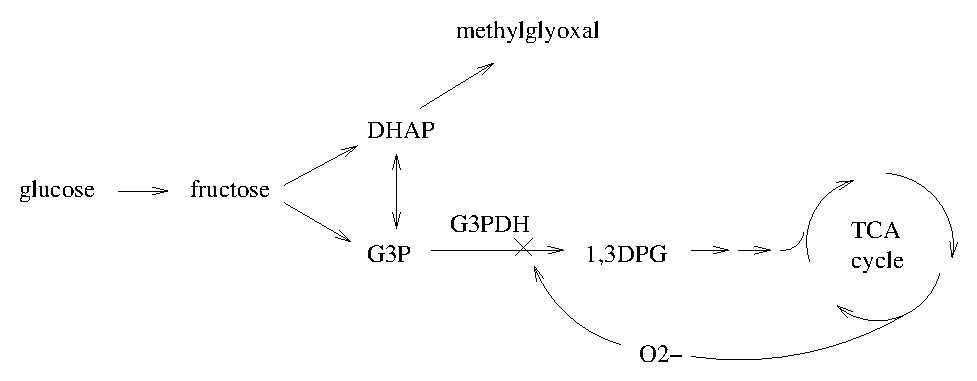
\includegraphics[width=0.75\textwidth]{figures/glycolysis} 

    in order to estimate rate parameters, predict responses to
    changes, and understand the system.
  \end{block}
}
\frame{
  \frametitle{Overview}
  \begin{block}{Method:}
    ``Wrap'' standard deterministic mathematical model
    within a Bayesian statistical model 
  \end{block}
}  

\section{Evaluation Approach}
\frame{
  \frametitle{Evaluation Approach}
  \begin{enumerate}
  \item{Create artificial model}
  \item{Generate artificial data}
  \item{Construct Mathematical + Bayesian Model}
  \item{Fit constructed model}
  \item{Compare results to known truth}
  \end{enumerate}
}

\section{Simulation Setup}
\subsection{Pathway Structure}
\frame{
  \frametitle{Pathway Structure}
  Relationship Diagram:
  \begin{reaction} source \yields R1 \yields R2 \yields
    R3 \yields R4 \yields R5 \yields sink \end{reaction}

  Chemical Equations:
  \begin{chemarray*} \small
    source &\yields^{k_1}& R1\\
    R1 + E1 &\eqbm^{k_2}_{k_3}& R1E1 \yields^{k_4} R2 + E1\\
    R2 + E2 &\eqbm^{k_5}_{k_6}& R2E2 \yields^{k_7} R3 + E2\\
    R3 + E3 &\eqbm^{k_8}_{k_9}& R3E3 \yields^{k_{10}} R4 + E3\\
    R4 + E4 &\eqbm^{k_{11}}_{k_{12}}& R4E4 \yields^{k_{13}} R5 + E4\\
    R5 &\yields^{k_{14}}& sink
  \end{chemarray*}
}

\subsection{Rate constants}
\frame{
  \frametitle{Rate constants}
  \begin{center}
    \begin{tabular}{c|r c c|r}
      rate constant & value & ~ & rate constant & value\\
      \cline{1-2}
      \cline{4-5}
      $k_1$ &  1.600  & ~ &  $k_8$ & 0.090 \\   
      $k_2$ &  0.540  & ~ &  $k_9$ & 4.560 \\   
      $k_3$ & 19.500  & ~ & $k_{10}$ & 1.400 \\
      $k_4$ &  2.125  & ~ & $k_{11}$ & 0.106 \\
      $k_5$ &  0.190  & ~ & $k_{12}$ & 3.670 \\
      $k_6$ &  8.460  & ~ & $k_{13}$ & 1.640 \\
      $k_7$ &  2.077  & ~ & $k_{14}$ & 0.400 \\
      \cline{1-2}
      \cline{4-5}
    \end{tabular}
  \end{center}
}

\subsection{Data Generation}
\frame{
  \frametitle{Data Generation}
  \begin{itemize}
  \item Use Gillespie's method to generate ``observed'' data
  \item Start at equilibrium
  \item Add bolus of $R1$ at time $20$.
    \vspace{-0.125in}
    \begin{center}
      \label{pulse}
      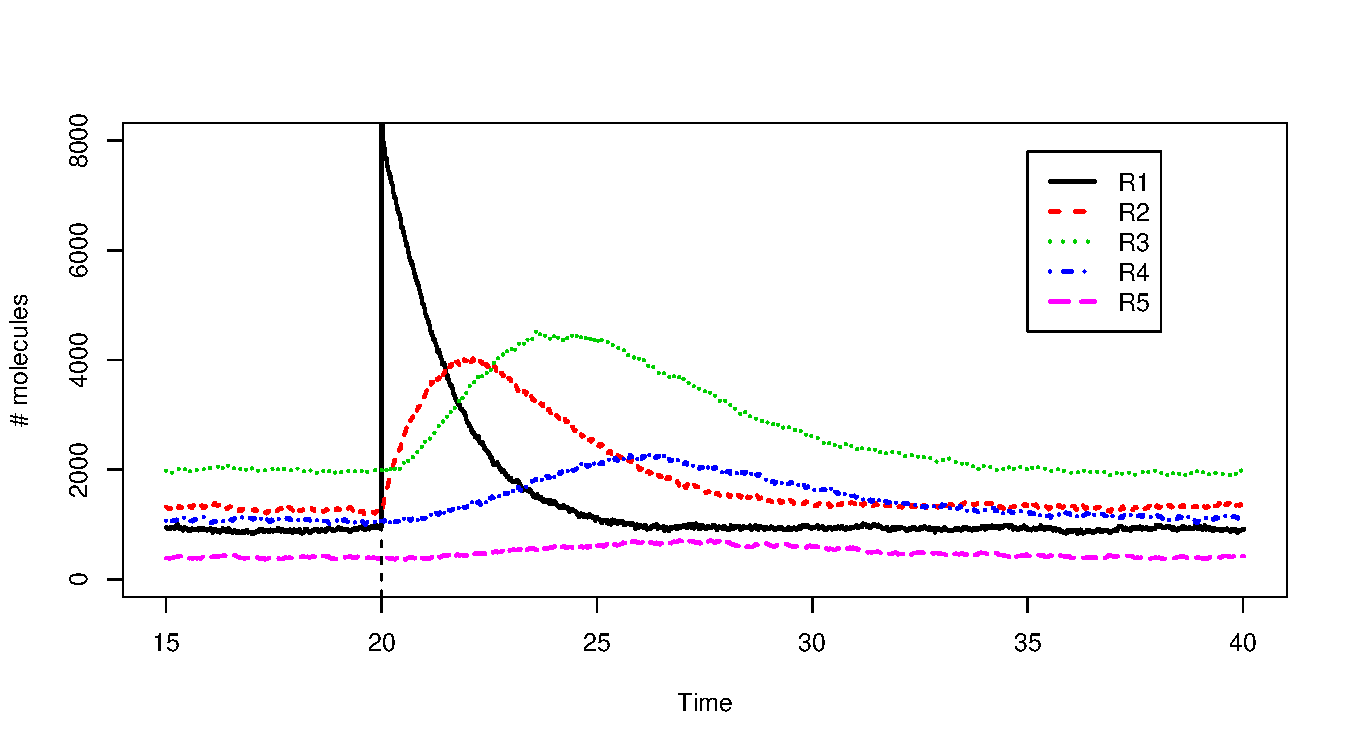
\includegraphics[height=0.6\textheight]{figures/pulse}
    \end{center}
    \vspace{-0.125in}
  \item Triplicate estimates of reactant concentrations every minute
  \item Estimate 'velocity' via locally linear smoother, avoiding spike..
  \end{itemize}

}
 
\section{Model Specification}

\subsection{What do we need?}
\frame{
  \frametitle{Model Specification: What do we need?}
  \begin{itemize}
  \item Relationship between parameters and observable data:
    \begin{itemize}
    \item Biochemical model
    \item Error structure
    \end{itemize}
  \item Priors for parameters
  \item Observed Data
  \item Fitting Method
  \end{itemize}
}
 
\subsection{Biochemical Models}
\frame{
  \frametitle{Michaelis-Menten}
  
  Individual reactions were fit using the Michaelis-Menten equation
  for individual enzymes. This is a reaction of the form
  \begin{reaction}\label{eqnForm}
    E + S \eqbm^{k_1}_{k_2} ES \yields^{k_3} E + P
  \end{reaction}
  where
  \begin{eqnarray*}
    S &=& \text{substrate concentration}\\
    E &=& \text{free enzyme concentration}\\
    ES &=& \text{concentration of the enzyme-substrate complex}\\
    P &=& \text{product concentration}
  \end{eqnarray*}
}

\frame{
  \frametitle{Steady State}
    In a steady state the rate
    of the reaction $v$ is
    \begin{equation}
    v = \frac{V_{max}S}{K_m+S} 
    \end{equation}
    where
    \begin{eqnarray*}
      V_{max} &=& (E+ES)k_3 = \text{maximum reaction velocity}\\[2mm]
      K_m &=& \frac{k_2+k_3}{k_1} = \text{substrate concentration at
      half-maximal velocity}
    \end{eqnarray*}
    This form of the equation is very useful because $v$ and $S$ are
    usually measurable and $V_{max}$ and $K_m$ can be obtained by
    fitting  equation 3 to the data. I

    %In contrast, modeling $v$ as a
%    function of the individual rate constants is less useful because
%    that requires the measurement of the concentration of the
%    enzyme-substrate complex which is technically difficult.
}

\frame{
  \frametitle{Non-steady state}
    In this application we are dealing with sequences of reactions
    which are not in a steady state, so we cannot use the
    Michaelis-Menten equation directly. Instead, we use equations
    of the form
    \begin{equation}
    v = \frac{aS}{b+S} - \frac{cP}{d+P} 
  \end{equation}
    
  The coefficients $a$, $b$, $c$, and $d$ in the equations can be
  estimated with data obtained following a change in the
  concentration of one of the reactants. For example, for the data
  plotted in Slide~\ref{pulse}:
    \begin{align*}
      \deriv{R2}{t} &= v_2 = \frac{d_1R1}{d_2 + R1} -
      \frac{d_3R2}{d_4 + R2}\\[5mm]
    \end{align*}
}


\subsection{Error distribution}

\frame{
  \frametitle{Error distribution}
  The error in the velocity estimates is assumed
  to be $N(0,\sigma^2)$ so that the reaction velocities $v_j$ have a
  normal distribution:
  \[
  v_j \sim N(\mu_j,\sigma^2)
  \]

  where
  \[
  \mu_j = \frac{aS_j}{b+S_j} - \frac{cP_j}{d+P_j} 
  \]
}

\frame{
  \frametitle{Likelihoods}
  Putting this together yields:
  \begin{align*}
    v_2 &\sim N\left(\frac{d_1R1}{d_2+R1} -
      \frac{d_3R2}{d_4+R2}, \;\; \sigma^2\right)\\
    v_3 &\sim N\left(\frac{d_3R2}{d_4+R2} -
      \frac{d_5R3}{d_6+R3}, \;\; \sigma^2\right)\\
    v_4 &\sim N\left(\frac{d_5R3}{d_6+R3} -
      \frac{d_7R4}{d_8+R4}, \;\; \sigma^2\right)\\
    \intertext{and}
    v_5 &\sim N\left(\frac{d_7R4}{d_8+R4} - d_9R5, \;\; \sigma^2\right)
  \end{align*}
}

\subsection{Prior Distributions}

\frame{
  \frametitle{Prior Distributions}

  For coefficients $d_1$ -- $d_5$: 
  \[
  \frac{3d_i}{\mu_i} \sim \chi_5^2
  \]
  where $\mu_i$ is a prior estimate of the parameter values.
  
  ~ 

  For $\sigma^2$:
  \[
  \sigma \equiv 2
  \]
  }

\section{Fitting}
\frame{
  \frametitle{Fitting algorithm}
  
  We applied 3 different MCMC algorithms (in order of shortest to
  longest required run length) as implemented in the \textsc{Hydra}
  MCMC library for \textsc{Java}.

  \begin{enumerate}
    \item Normal Kernel Coupler
    \item Multivariate normal increment Metropolis
    \item Univariate normal increment Metropolis
  \end{enumerate}
  
  Convergence and required run-length was estimated using
  \textsc{mcgibbsit}, using $q=0.025$, $r=0.0125$, and $s=0.95$,
  which ensure reliable confidence intervals. 
}

\frame{
  \frametitle{Convergence Rates}
  \begin{center}
    Mean Squared Residuals \\
    ~

    \begin{tabular}{c||c|c|c||c|c|c}
       &
       \multicolumn{3}{c||}{mean residual SSQ $\times 10^{-4}$} & \multicolumn{3}{c}{$R_{adj}^2$}\\
      \cline{2-7}
      algorithm & 12 pt. & 16 pt. & 25 pt. &
      12 pt. & 16 pt. & 25 pt.\\
      \hline
       1-comp & 1.34 & 0.83 & 1.06 & 0.87 & 0.92 & 0.86\\
       all-comp & 0.74 & 0.93 & 0.74 & 0.93 & 0.90 & 0.90 \\
       NKC & 0.86 & 0.73 & 0.71 & 0.92 & 0.92 & 0.91
    \end{tabular}
  \end{center}
}

\section{Results}
\frame{
  \frametitle{Results}
  
  
  \begin{columns}[c]
  \column{2in} 

  Bivariate scatter plots of the parameter distributions (upper
  triangle) and correlation coefficients (lower triangle). 

  ~

  Note the strong correlation between some pairs of parameters,
  e.g., $d_1$ -- $d_2$.

  \column{2in}

  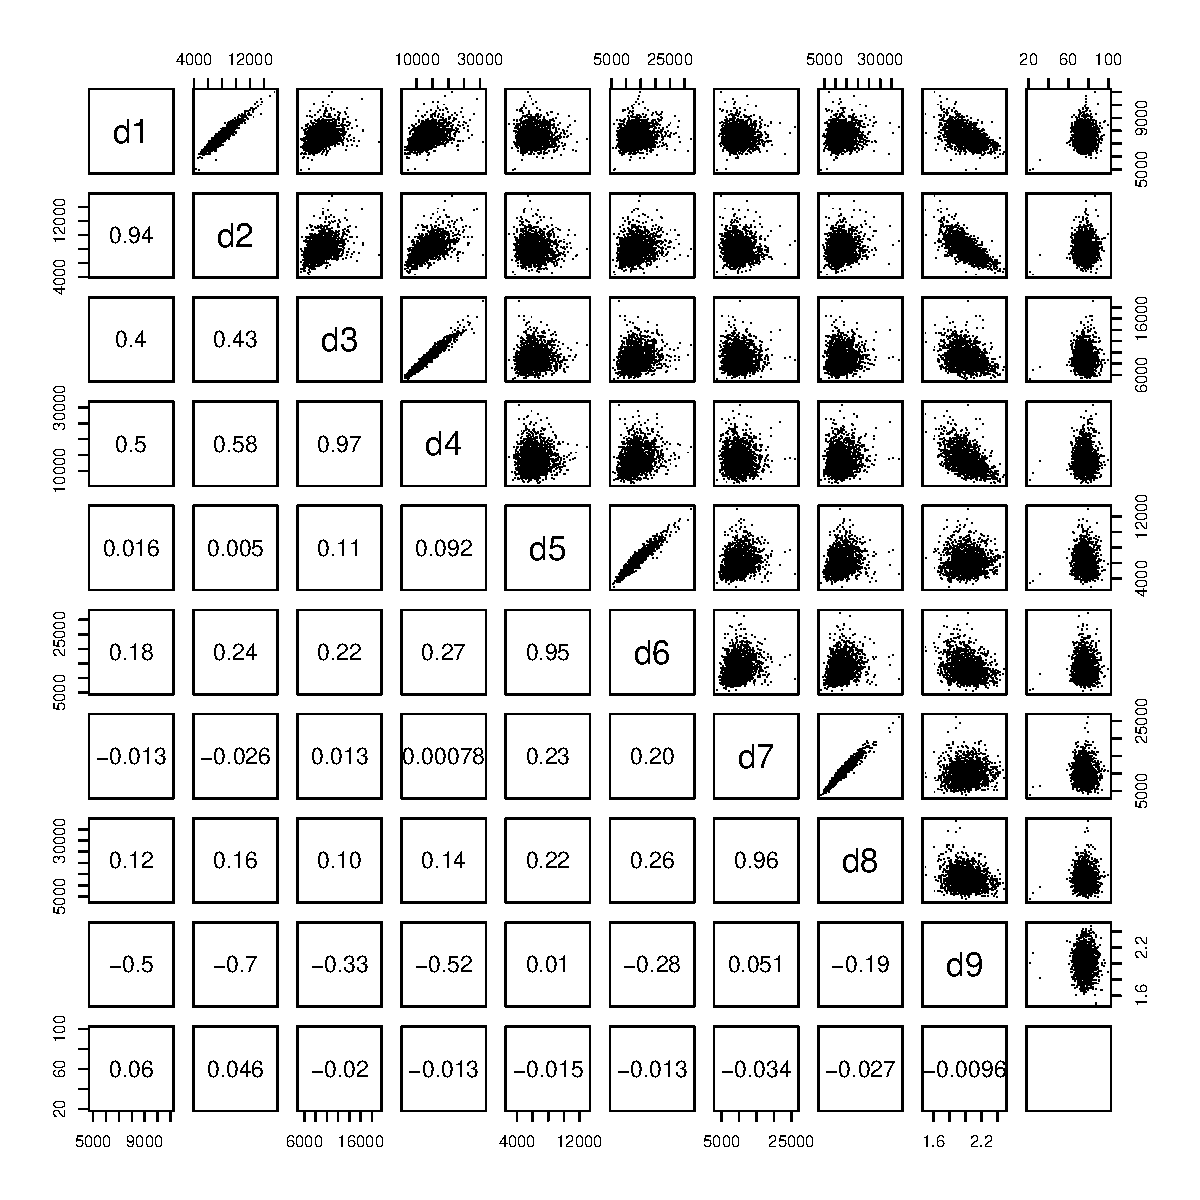
\includegraphics[width=2in]{figures/scatterPlot}
  \end{columns}
}

\frame{
  \frametitle{Actual vs Fitted}

  \begin{center}
  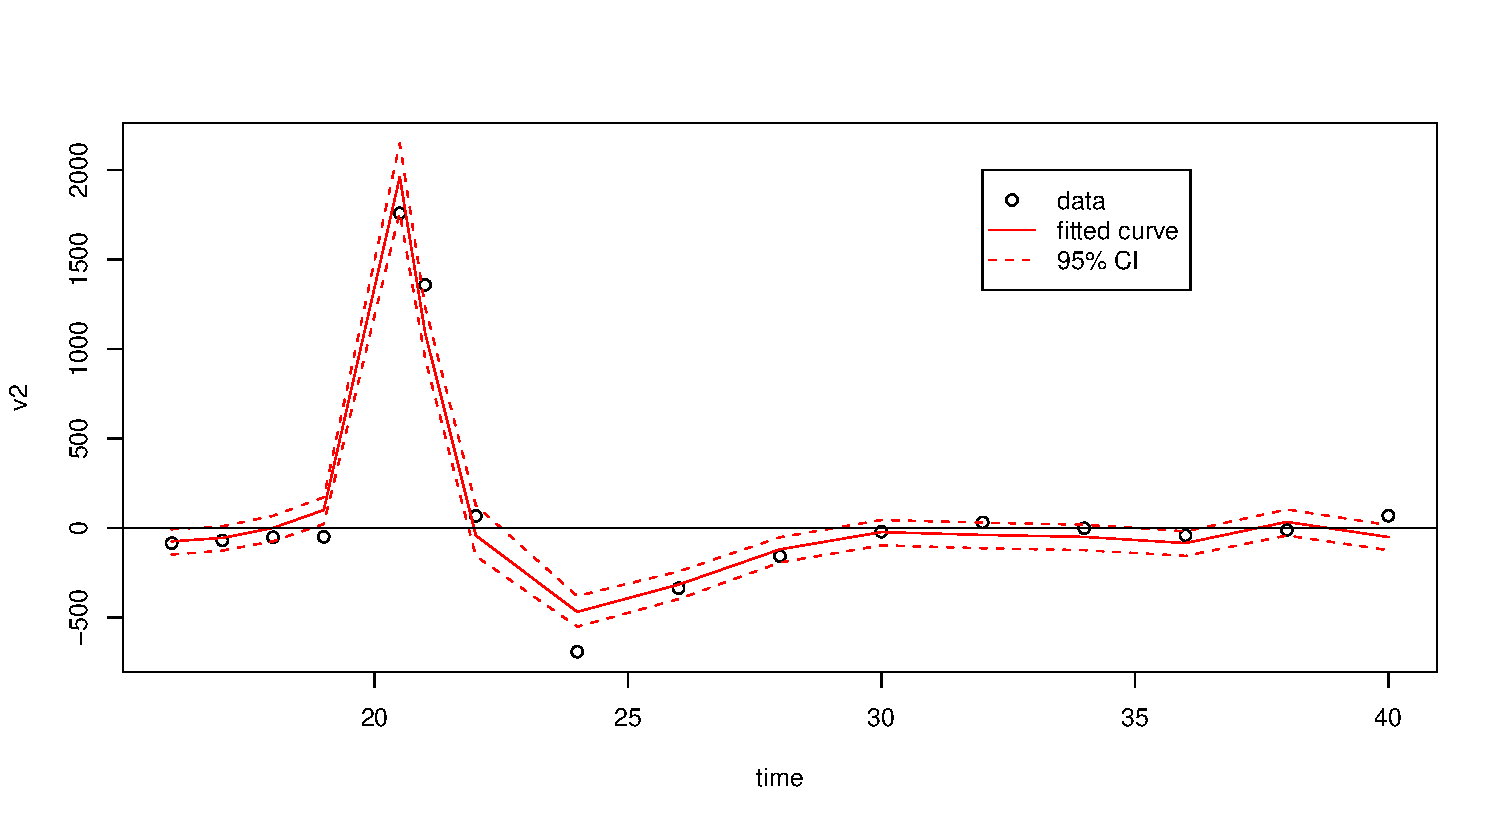
\includegraphics[width=0.5\textwidth]{figures/V1fitted}
  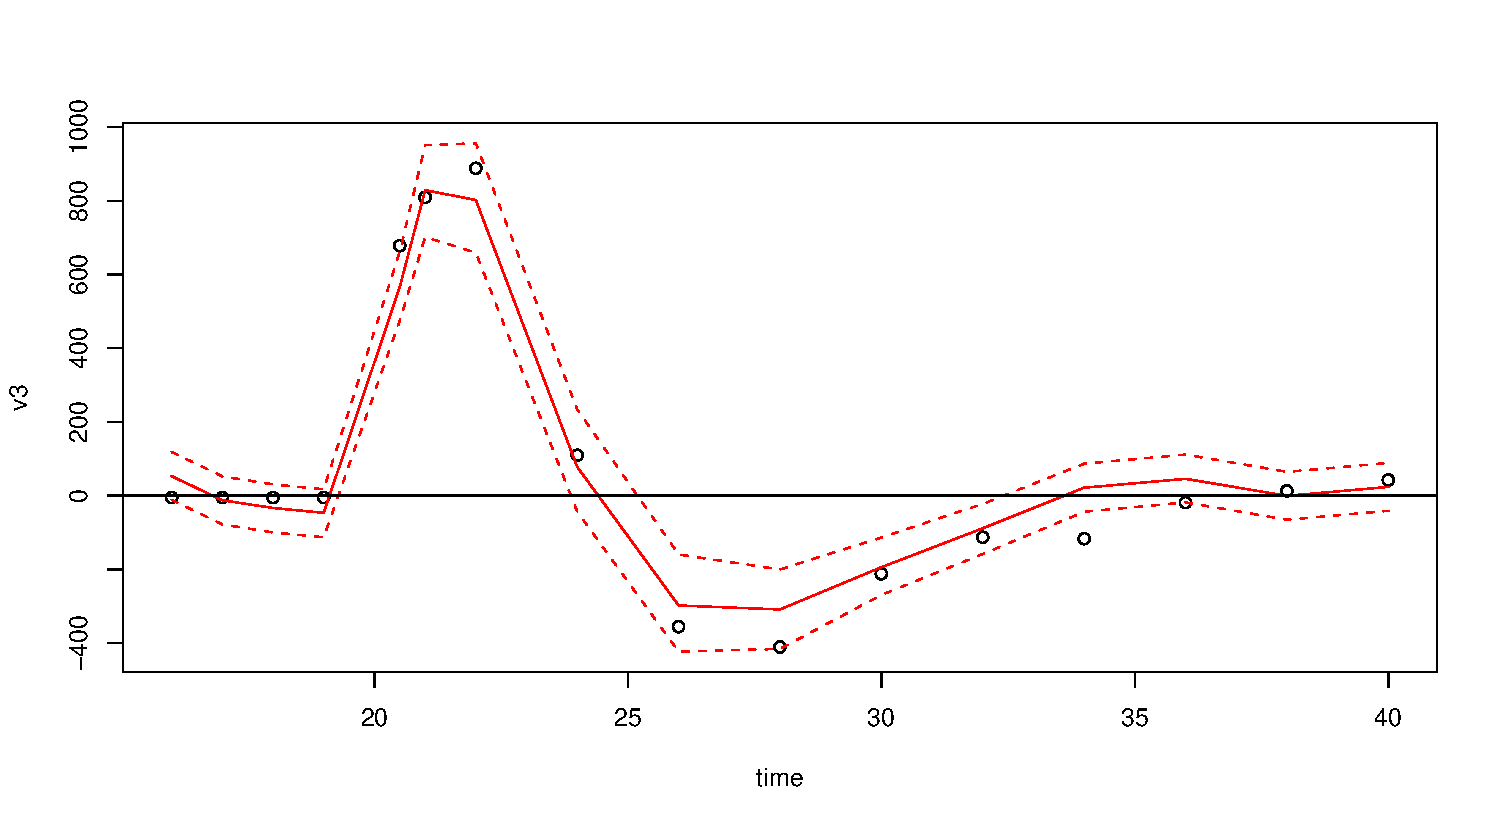
\includegraphics[width=0.5\textwidth]{figures/V2fitted} \\

  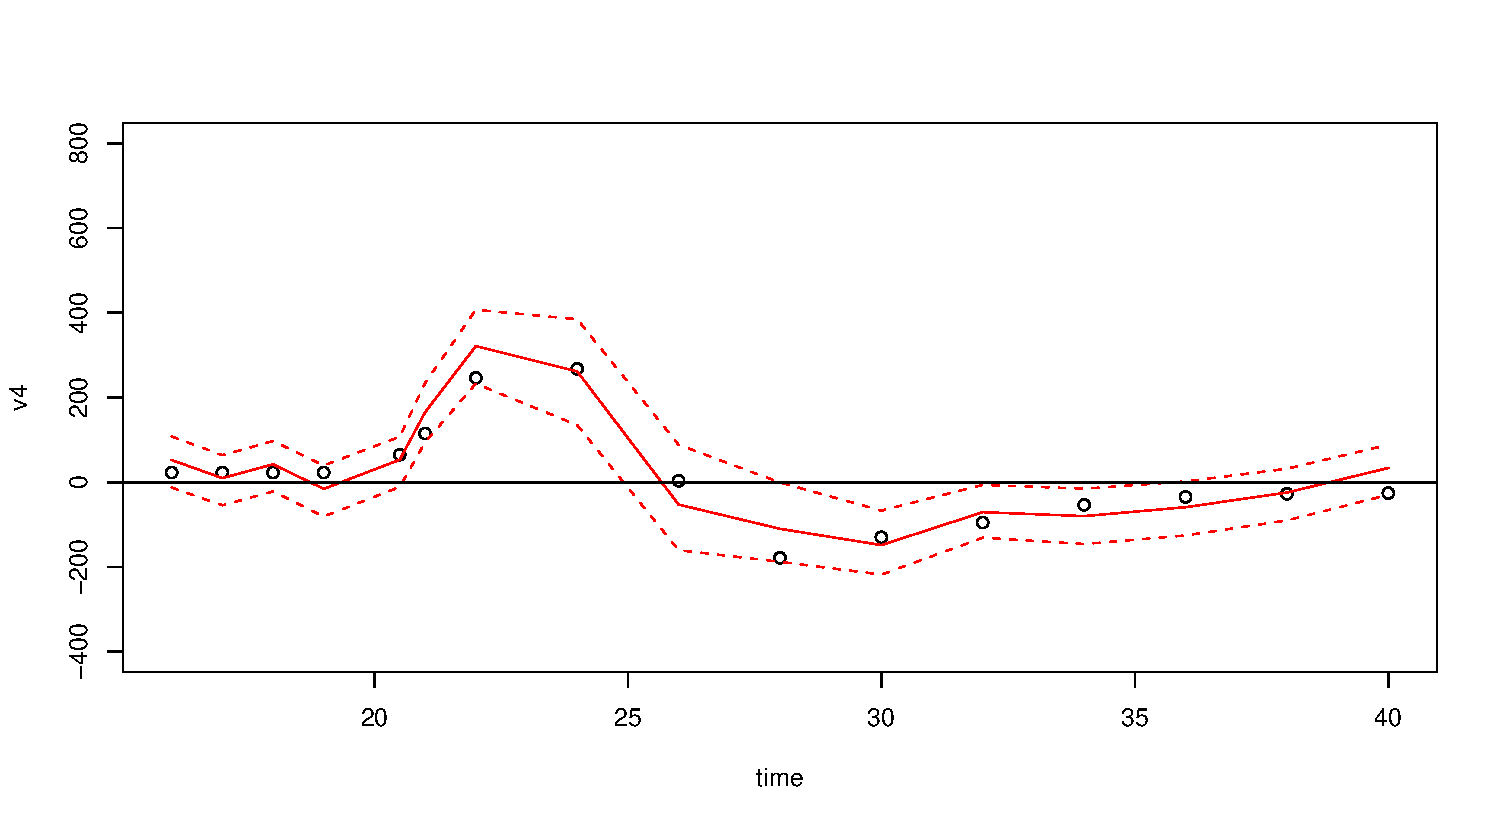
\includegraphics[width=0.5\textwidth]{figures/V3fitted}
  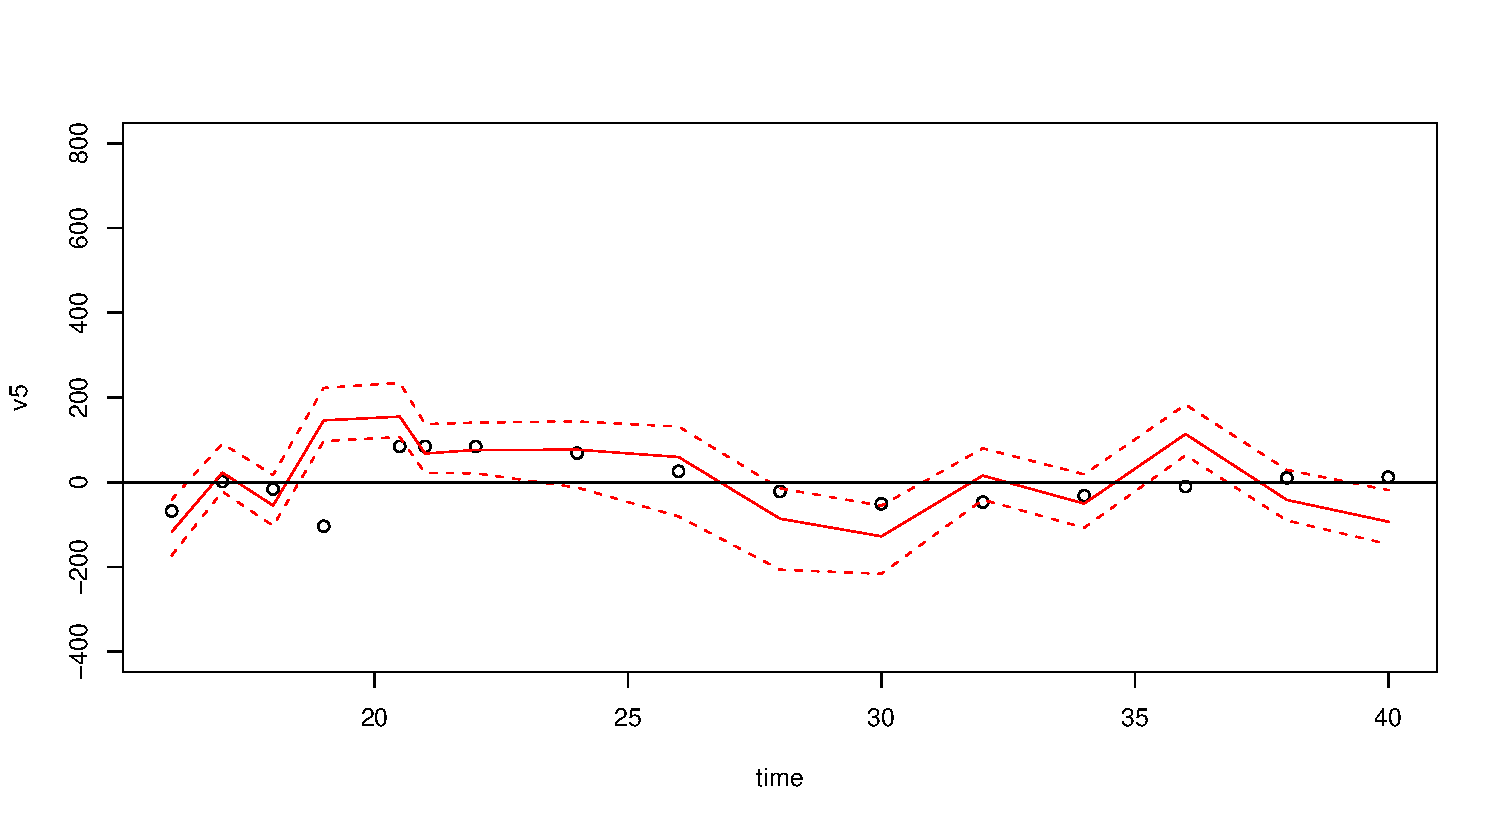
\includegraphics[width=0.5\textwidth]{figures/V4fitted} \\
  \end{center}
}

\section[]{References}
\frame{
  \frametitle{For More Information}
  \begin{itemize}
  \item Greg Warnes \
    \begin{itemize}
    \item Email: \texttt{gregory.r.warnes@pfizer.com}
    \item Personal Web Page: \textt{http://www.warnes.net}
    \item Research Web Page: \textt{http://research.warnes.net}
    \end{itemize}
  \item Robert Burrows 
    \begin{itemize}
    \item Email: \texttt{rbb@nebiometrics.com}
    \item Web Page: \textt{http://www.nebiometrics.com}
    \end{itemize}
  \end{itemize}
}

\end{document}
